\documentclass[11pt]{amsart}

\usepackage[T1]{fontenc}
\usepackage{lmodern}
\usepackage{amssymb,amsmath}
\usepackage{graphicx}
\usepackage{booktabs}
\usepackage{array}
\usepackage{xcolor}
\usepackage[margin=1.15in]{geometry}
\usepackage[colorlinks=true,linkcolor=blue!50!black,citecolor=blue!50!black,urlcolor=blue!50!black]{hyperref}

\newtheorem{theorem}{Theorem}[section]
\newtheorem{proposition}[theorem]{Proposition}
\newtheorem{lemma}[theorem]{Lemma}
\newtheorem{corollary}[theorem]{Corollary}
\newtheorem{conjecture}[theorem]{Conjecture}
\theoremstyle{definition}
\newtheorem{definition}[theorem]{Definition}
\newtheorem{question}[theorem]{Question}
\theoremstyle{remark}
\newtheorem{remark}[theorem]{Remark}

\numberwithin{equation}{section}

\newcommand{\doi}[1]{\href{https://doi.org/#1}{\nolinkurl{doi:#1}}}
\newcommand{\ggr}{\gamma_{\mathrm{gr}}}
\newcommand{\sprod}{\boxtimes}
\newcommand{\oct}{K_{2,2,2}}
\hypersetup{pdftitle={The Grundy domination number is not multiplicative on strong products},pdfauthor={Deep Bhattacharjee}}

\begin{document}

\title[Grundy domination of strong products]{The Grundy domination number is not\\ multiplicative on strong products}

\author{Deep Bhattacharjee}
\address{Formerly, Electro-Gravitational Space Propulsion Laboratory (EGSPL),\newline Bhubaneswar, Odisha 751030, India}
\email{d.bhattacharjee@erl-forschung.de}
\email{itsdeep@live.com}
\urladdr{https://orcid.org/0000-0003-0466-750X}
\thanks{Corresponding author: \href{mailto:d.bhattacharjee@erl-forschung.de}{d.bhattacharjee@erl-forschung.de}; ORCID \href{https://orcid.org/0000-0003-0466-750X}{\mbox{0000-0003-0466-750X}}}

\subjclass[2020]{Primary 05C69; Secondary 05C76}
\keywords{Grundy domination number, dominating sequence, strong product, circular clique, formal verification}

\begin{abstract}
The strong product of the octahedron with a graph $H$ on $21$ vertices of Grundy domination number $10$ has Grundy domination number at least $21$. This disproves the conjecture of Bre\v{s}ar, Bujt\'as, Gologranc, Klav\v{z}ar, Ko\v{s}mrlj, Patk\'os, Tuza and Vizer that $\ggr(G\sprod H)=\ggr(G)\ggr(H)$ for all graphs $G$ and $H$.
\end{abstract}

\maketitle

\section{Introduction}

Let $G$ be a finite simple graph and write $N[v]$ for the closed neighbourhood of a vertex $v$. A sequence $(v_1,\dots,v_k)$ of vertices of $G$ is \emph{legal} if every $v_i$ dominates a vertex not dominated by its predecessors, that is,
\[
  N[v_i]\setminus\bigcup_{j<i}N[v_j]\neq\emptyset\qquad(1\le i\le k);
\]
a vertex in this difference is a \emph{footprint} of $v_i$. The vertices of a legal sequence are distinct. The \emph{Grundy domination number} $\ggr(G)$ is the length of a longest legal sequence; a longest legal sequence always dominates $G$. The parameter was introduced by Bre\v{s}ar, Gologranc, Milani\v{c}, Rall and Rizzi~\cite{BGMRR}, who connected it with the domination game.

In the strong product $G\sprod H$ two distinct vertices $(g,h)$ and $(g',h')$ are adjacent when $g'\in N_G[g]$ and $h'\in N_H[h]$; equivalently $N_{G\sprod H}[(g,h)]=N_G[g]\times N_H[h]$. Taking a Grundy dominating sequence of $G$ and one of $H$ and listing their pairs in lexicographic order gives a legal sequence of $G\sprod H$, so
\begin{equation}\label{eq:lower}
  \ggr(G\sprod H)\ \ge\ \ggr(G)\,\ggr(H)
\end{equation}
for all $G$ and $H$~\cite[Proposition~21]{BBG}. In the same paper the authors conjectured that the bound is always attained.

\begin{conjecture}[{\cite[Conjecture~22]{BBG}}]\label{conj}
For all graphs $G$ and $H$, $\ggr(G\sprod H)=\ggr(G)\,\ggr(H)$.
\end{conjecture}

The conjecture holds when $G$ is a caterpillar~\cite{BBG} and, more generally, when $G$ is a forest, by the work of Bell, Driscoll, Krop and Wolff~\cite{BDKW}. A proof for all graphs was announced by Herrman and Smith~\cite{HS} and later withdrawn.\footnote{The second version of arXiv:2212.04565 (12 January 2023) carries the comment ``There is an error. Some cases were not considered in the proof of Theorem~1.''} We show that the conjecture is false.

For $N\ge1$ let $H_N$ be the graph on $\{0,1,\dots,N-1\}$ in which $u$ and $v$ are adjacent when $|u-v|\equiv2\pmod 3$. Let $\oct$ be the octahedron, the complete tripartite graph with three parts of size two.

\begin{theorem}\label{thm:main}
$\ggr(\oct)=2$, $\ggr(H_{21})=10$ and $\ggr(\oct\sprod H_{21})\ge21$. In particular
\[
  \ggr(\oct\sprod H_{21})\ >\ \ggr(\oct)\,\ggr(H_{21}),
\]
and Conjecture~\ref{conj} fails.
\end{theorem}

The lower bound for the product is a short explicit argument valid for every $N$ (Proposition~\ref{prop:product}), and so is $\ggr(\oct)=2$ (Lemma~\ref{lem:oct}). The upper bound $\ggr(H_{21})\le10$ is the one step that rests on a finite computation: an exhaustive search through the sets dominated by legal sequences, which we have certified in the Lean~4 proof assistant~\cite{MU} (Section~\ref{sec:H21}). The same search gives a family of counterexamples.

\begin{theorem}\label{thm:family}
For every $N\ge1$, $\ggr(\oct\sprod H_N)\ge N$. For $6\le N\le 63$,
\[
  \ggr(H_N)=\Big\lfloor\frac{N+1}{3}\Big\rfloor+3 ,
\]
so $\ggr(\oct\sprod H_N)>\ggr(\oct)\,\ggr(H_N)$ for $21\le N\le 63$. For $N=63$ the ratio $\ggr(\oct\sprod H_N)/\big(\ggr(\oct)\ggr(H_N)\big)$ is at least $63/48=21/16$.
\end{theorem}

The second statement of Theorem~\ref{thm:family} is computational (Section~\ref{sec:family}); the first is Proposition~\ref{prop:product}. If the formula for $\ggr(H_N)$ holds for all $N$, the ratio approaches $3/2$. By Proposition~25 of~\cite{BBG}, $\ggr(G\sprod H)\le|V(G)|\,\ggr(H)$, so for $G=\oct$ the ratio can never exceed $3$.

\section{The graphs}\label{sec:graphs}

We write the vertices of the octahedron as $g_0,g_1,g_2,x_0,x_1,x_2$ (in this order, $0,\dots,5$), where $x_t$ is the antipode of $g_t$; the three antipodal pairs are the only non-adjacent pairs (Figure~\ref{fig:oct}). Thus $N[v]$ is everything except the antipode of $v$.

\begin{figure}[ht]
\centering
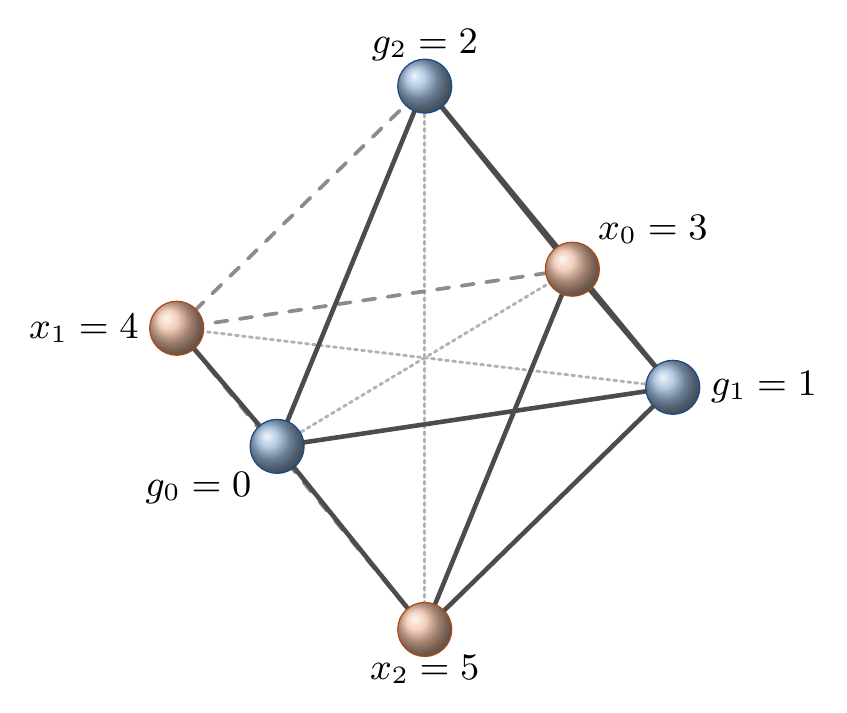
\includegraphics[width=0.42\textwidth]{figures/octahedron.png}
\caption{The octahedron $\oct$. Each vertex is adjacent to all others except its antipode; the dotted segments join the antipodal pairs $\{g_t,x_t\}$.}\label{fig:oct}
\end{figure}

\begin{lemma}\label{lem:oct}
$\ggr(\oct)=2$.
\end{lemma}

\begin{proof}
The sequence $(g_0,x_0)$ is legal: $x_0$ footprints itself. Conversely, let $(u,v)$ be legal. If $v$ is the antipode of $u$, then $N[u]\cup N[v]$ is the whole vertex set; otherwise $N[u]$ misses only the antipode of $u$, which lies in $N[v]$. Either way nothing is left for a third vertex to footprint.
\end{proof}

In $H_N$ we write $a_i=3i$, $b_i=3i+1$ and $c_i=3i+2$. Two vertices of the same residue class are never adjacent, and for vertices of different classes,
\begin{equation}\label{eq:adj}
  a_i\sim c_j\iff j\ge i,\qquad b_i\sim a_j\iff j>i,\qquad c_i\sim b_j\iff j>i,
\end{equation}
because $c_j-a_i=3(j-i)+2$, $a_j-b_i=3(j-i)-1$ and $b_j-c_i=3(j-i)-1$. When $N=3n$ the graph has a circular description (Figure~\ref{fig:ring}). Recall that the circular clique $K_{p/q}$ has vertex set $\mathbb Z_p$, two vertices being adjacent when their cyclic distance is at least $q$.

\begin{proposition}\label{prop:circular}
Let $n\ge2$ and place the vertices of $H_{3n}$ on a cycle in the order
\[
  a_0,\dots,a_{n-1},\ c_0,\dots,c_{n-1},\ b_0,\dots,b_{n-1}.
\]
Two vertices are adjacent in $H_{3n}$ if and only if their cyclic distance is at least $n+1$, or they are $a_i$ and $c_i$ for some $i$. Thus $H_{3n}$ is the circular clique $K_{3n/(n+1)}$ together with the perfect matching $\{a_ic_i\}$.
\end{proposition}

\begin{proof}
Give $a_i$, $c_i$ and $b_i$ the positions $i$, $n+i$ and $2n+i$ modulo $3n$. Vertices of the same class are at cyclic distance at most $n-1$ and are not adjacent. For two vertices of different classes, name them so that the second follows the first in the cyclic order $A\to C\to B\to A$ of the blocks: the pairs are $(a_i,c_j)$, $(c_i,b_j)$ and $(b_i,a_j)$. In each case the second position minus the first is $n+(j-i)$ modulo $3n$, with $|j-i|\le n-1$, so the cyclic distance is at least $n+1$ when $j>i$, exactly $n$ when $j=i$, and at most $n-1$ when $j<i$. Comparing with~\eqref{eq:adj}: the pair is adjacent exactly when $j>i$, except that $a_i\sim c_i$.
\end{proof}

\begin{figure}[ht]
\centering
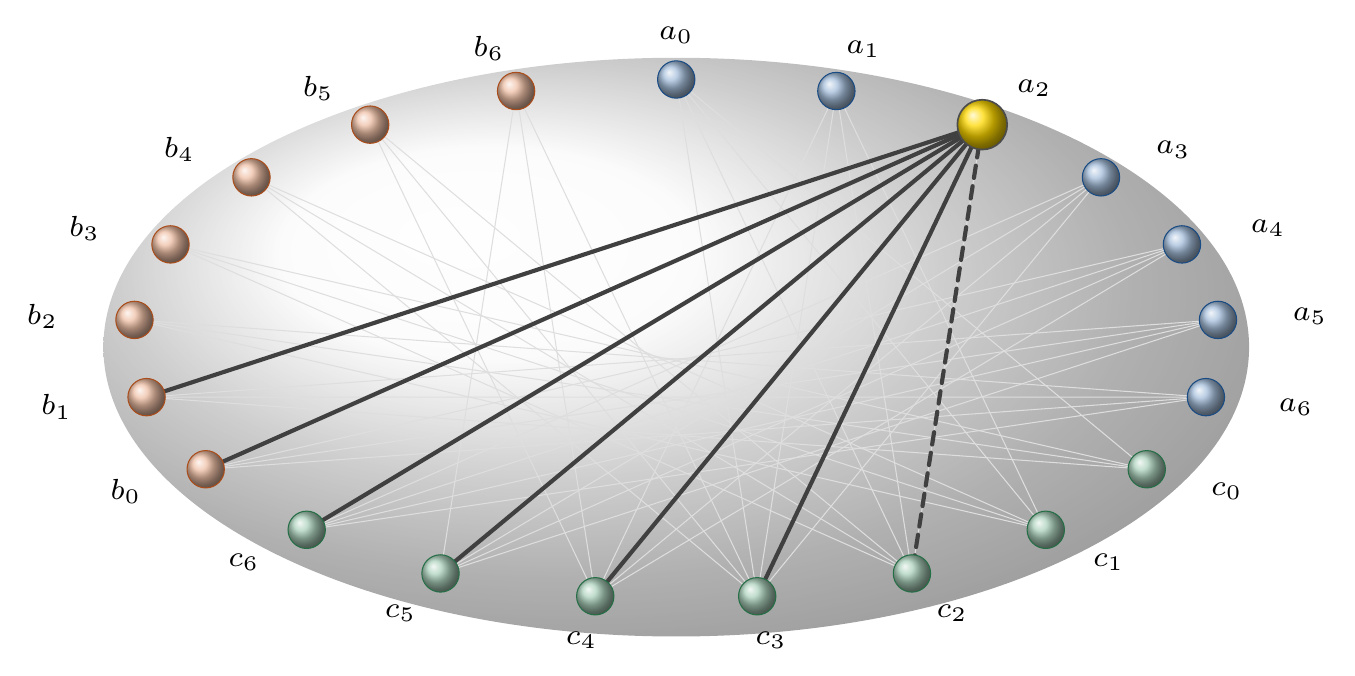
\includegraphics[width=0.78\textwidth]{figures/ring.png}
\caption{$H_{21}$ on a ring in the order of Proposition~\ref{prop:circular}; all edges are drawn faintly. The closed neighbourhood of $a_2$ is $a_2$ together with the arc $c_3,\dots,c_6,b_0,b_1$ of vertices at cyclic distance at least $8$ and its partner $c_2$ (dashed).}\label{fig:ring}
\end{figure}

\section{A long legal sequence in the product}\label{sec:product}

The construction uses one property of $H_N$: with the colouring $v\mapsto v\bmod 3$, every edge $uv$ with $u<v$ satisfies $u\equiv v+1\pmod 3$. We state it for any graph with this property.

\begin{proposition}\label{prop:product}
Let $H$ be a graph with vertices $v_0,\dots,v_{N-1}$ and a map $t\colon V(H)\to\mathbb Z_3$ such that $t(v_i)\equiv t(v_j)+1\pmod3$ for every edge $v_iv_j$ with $i<j$. Then the sequence
\[
  s_j=\big(g_{t(v_j)},\,v_j\big),\qquad j=0,1,\dots,N-1,
\]
is legal in $\oct\sprod H$, and $\ggr(\oct\sprod H)\ge N$. In particular $\ggr(\oct\sprod H_N)\ge N$ for every $N\ge1$, with $t(v)=v\bmod3$.
\end{proposition}

\begin{proof}
We show that $s_j$ footprints $f_j=(x_{t(v_j)+1},v_j)$, indices of $g$ and $x$ taken modulo $3$. First, $f_j\in N[s_j]$: the vertex $x_{t(v_j)+1}$ is not the antipode $x_{t(v_j)}$ of $g_{t(v_j)}$, so it lies in $N[g_{t(v_j)}]$, and $v_j\in N[v_j]$. Now let $i<j$. If $f_j\in N[s_i]$, then $x_{t(v_j)+1}\in N[g_{t(v_i)}]$, which means $t(v_i)\ne t(v_j)+1$, and $v_j\in N[v_i]$, which for $i\neq j$ means that $v_iv_j$ is an edge, hence $t(v_i)=t(v_j)+1$. The two conclusions contradict each other, so $f_j\notin N[s_i]$.
\end{proof}

Figure~\ref{fig:product} shows the sequence for $H_{21}$. Every column of the product contains exactly one vertex of the sequence, while a Grundy dominating sequence of the form used for~\eqref{eq:lower} would use only $\ggr(H_{21})=10$ columns. The rotation of the three colours along the sequence is what lets each new vertex reach a footprint in a layer $x_t$ that none of the earlier vertices covers in that column.

\begin{figure}[ht]
\centering
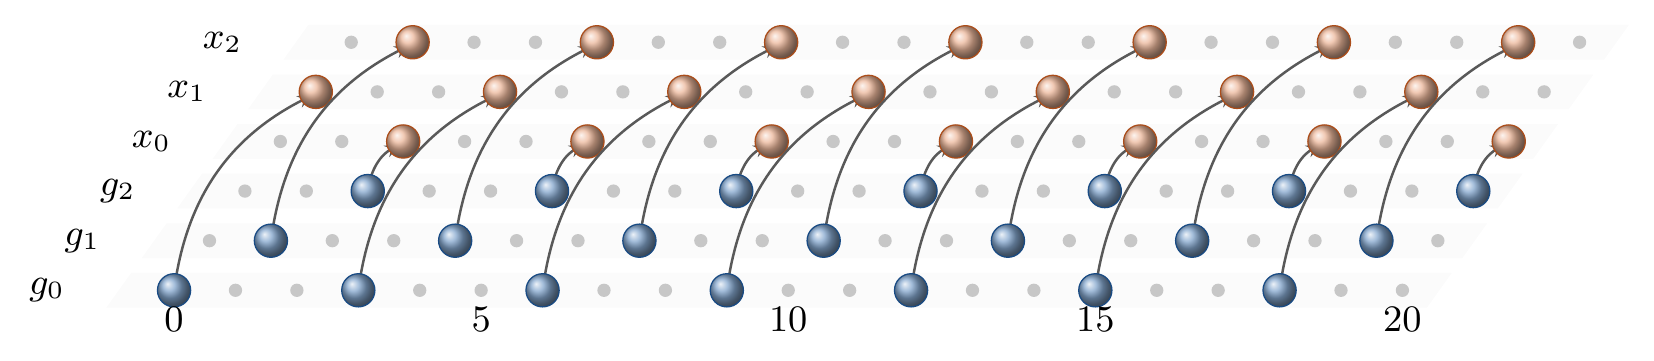
\includegraphics[width=\textwidth]{figures/product.png}
\caption{$\oct\sprod H_{21}$ as six stacked copies of $H_{21}$, one for each vertex of the octahedron. The $21$ blue vertices $(g_{j\bmod3},j)$ form a legal sequence; the arrow from each of them ends at its footprint $(x_{(j+1)\bmod 3},j)$.}\label{fig:product}
\end{figure}

\section{The Grundy domination number of \texorpdfstring{$H_{21}$}{H21}}\label{sec:H21}

\begin{lemma}\label{lem:h21lower}
$\ggr(H_{21})\ge10$.
\end{lemma}

\begin{proof}
The sequence $(a_0,a_1,a_2,a_3,a_4,b_6,c_4,c_0,a_5,b_0)$, that is $(0,3,6,9,12,19,14,2,15,1)$, is legal and dominating. By~\eqref{eq:adj}, $a_0$ dominates $c_0,\dots,c_6$; each $a_i$ with $1\le i\le4$ footprints itself and $b_{i-1}$; then $b_6$ footprints itself, $c_4$ footprints $b_5$, $c_0$ footprints $b_4$, $a_5$ footprints itself and $b_0$ footprints $a_6$.
\end{proof}

For the upper bound we use the sets of dominated vertices. For a legal sequence $S=(v_1,\dots,v_k)$ put $D(S)=N[v_1]\cup\dots\cup N[v_k]$. Define families $\mathcal L_0,\mathcal L_1,\dots$ of vertex sets by $\mathcal L_0=\{\emptyset\}$ and
\[
  \mathcal L_{k+1}=\big\{\,D\cup N[v]\;:\;D\in\mathcal L_k,\ v\in V(G),\ N[v]\not\subseteq D\,\big\}.
\]

\begin{lemma}\label{lem:layers}
If $S$ is a legal sequence of length $k$, then $D(S)\in\mathcal L_k$. Hence $\ggr(G)$ is the largest $k$ with $\mathcal L_k\neq\emptyset$.
\end{lemma}

\begin{proof}
Induction on $k$: if $(v_1,\dots,v_{k+1})$ is legal, then $D=D(v_1,\dots,v_k)\in\mathcal L_k$ and $N[v_{k+1}]\not\subseteq D$, so $D\cup N[v_{k+1}]\in\mathcal L_{k+1}$. Conversely, every member of $\mathcal L_k$ is $D(S)$ for a legal sequence $S$ of length $k$, by the same induction.
\end{proof}

The families can be large in general, but for $H_{21}$ they are small: by~\eqref{eq:adj}, the vertices of a class dominated by the vertices of another class form an initial or a final segment of that class.\footnote{For instance, the vertices $c_j$ dominated by the chosen vertices of the class $a$ are those with $j\ge\min\{i: a_i\text{ chosen}\}$.} Their sizes are
\[
  |\mathcal L_0|,\dots,|\mathcal L_{10}| = 1,\ 21,\ 210,\ 1023,\ 1482,\ 1302,\ 848,\ 419,\ 150,\ 22,\ 1,
\]
and $\mathcal L_{11}=\emptyset$; the only member of $\mathcal L_{10}$ is the whole vertex set. With Lemma~\ref{lem:layers} this gives the following.

\begin{proposition}\label{prop:h21upper}
$\ggr(H_{21})\le10$.
\end{proposition}

We have verified Proposition~\ref{prop:h21upper} in three independent ways. In Lean~4, a certificate lists the $5479$ sets of the families $\mathcal L_0,\dots,\mathcal L_{10}$ as bit masks stored in binary search trees, and the kernel checks by evaluation that $\emptyset\in\mathcal L_0$, that $D\cup N[v]\in\mathcal L_{k+1}$ for every $D\in\mathcal L_k$ and every $v$ with $N[v]\not\subseteq D$, and that no member of $\mathcal L_{10}$ has a proper extension. A formal version of Lemma~\ref{lem:layers}, proved in Lean for every graph and every such certificate, then bounds the length of every legal sequence of $H_{21}$ by $10$. The Lean statement uses the definitions of legal sequences, of $H_{21}$, of $\oct$ and of the strong product given in this paper, and the main theorem
\begin{quote}\small
\texttt{strong\_product\_counterexample}: there is a dominating legal sequence of length $21$ in $\oct\sprod H_{21}$, every legal sequence of $\oct$ has length at most $2$, every legal sequence of $H_{21}$ has length at most $10$, and $2\cdot10<21$
\end{quote}
depends only on the standard axioms \texttt{propext} and \texttt{Quot.sound}; no \texttt{native\_decide} is used. Independently, a C program computes the families by breadth-first search, and a Python program finds $\ggr(H_{21})=10$ by a memoised depth-first search over dominated sets; both use only the definition of $H_{21}$.

\begin{proof}[Proof of Theorem~\ref{thm:main}]
Lemma~\ref{lem:oct}, Lemma~\ref{lem:h21lower} with Proposition~\ref{prop:h21upper}, and Proposition~\ref{prop:product} with $N=21$.
\end{proof}

\section{The family \texorpdfstring{$H_N$}{HN}}\label{sec:family}

The same breadth-first search, run for $6\le N\le 63$, gives the values in Table~\ref{tab:values}; for $N\le24$ they agree with the depth-first search. With Proposition~\ref{prop:product} this proves Theorem~\ref{thm:family}.\footnote{Grundy domination numbers add over disjoint unions, and $G\sprod(H\cup H')=(G\sprod H)\cup(G\sprod H')$, so disjoint copies of $H_{21}$ already give infinitely many counterexamples, all with ratio $21/20$.} The largest search, for $N=63$, visits $193\,131\,321$ dominated sets and takes about five minutes on one core. The upper bound for $N=21$ is the only one we have checked in Lean.

\begin{table}[ht]
\centering
\caption{$\ggr(H_N)=\lfloor (N+1)/3\rfloor+3$ for $6\le N\le63$, by exhaustive search. The conjecture fails for $\oct\sprod H_N$ when $N>2\ggr(H_N)$, that is, for $N\ge21$.}\label{tab:values}
\small
\begin{tabular}{@{}c*{12}{c}@{}}
\toprule
$N$ & $6$--$7$ & $8$--$10$ & $11$--$13$ & $14$--$16$ & $17$--$19$ & $20$--$22$ & $23$--$25$ & $26$--$28$ & $29$--$31$ & $\cdots$ & $59$--$61$ & $62$--$63$\\
$\ggr(H_N)$ & $5$ & $6$ & $7$ & $8$ & $9$ & $10$ & $11$ & $12$ & $13$ & $\cdots$ & $23$ & $24$\\
\bottomrule
\end{tabular}
\end{table}

\begin{question}\label{q:formula}
Is $\ggr(H_N)=\lfloor (N+1)/3\rfloor+3$ for every $N\ge6$? An affirmative answer would give $\sup_{G,H}\ggr(G\sprod H)/\big(\ggr(G)\ggr(H)\big)\ge3/2$.
\end{question}

\begin{question}\label{q:sup}
Is $\ggr(G\sprod H)/\big(\ggr(G)\ggr(H)\big)$ bounded over all graphs $G$ and $H$? Which graphs $G$ satisfy Conjecture~\ref{conj} for every $H$? By~\cite{BDKW} all forests do, and Theorem~\ref{thm:main} shows that $\oct$ does not.
\end{question}

\begin{remark}
Deleting the matching $\{a_ic_i\}$ from $H_{3n}$ leaves the circular clique $K_{3n/(n+1)}$ (Proposition~\ref{prop:circular}), a circulant graph, and it still satisfies the hypothesis of Proposition~\ref{prop:product}. Our search gives $\ggr(K_{3n/(n+1)})=n+4$ for $3\le n\le11$, one more than $\ggr(H_{3n})$. Hence $\oct\sprod K_{27/10}$, $\oct\sprod K_{30/11}$ and $\oct\sprod K_{33/12}$ are counterexamples as well, with a vertex-transitive second factor; the matching only makes the counterexamples smaller.
\end{remark}

\subsection*{Computations and formal verification}
The Lean development, the C and Python programs, their outputs and the scripts that rebuild this paper are in the archive~\cite{Ar}. The Lean files (Lean~4.34.1, no external libraries) contain $25$ theorems; all of them depend only on the standard axioms.

\subsection*{Use of generative AI}
The author used Claude (Anthropic) to check the results by computer and in Lean and to help draft the text; the author verified every step and is responsible for the content.

\begin{thebibliography}{9}

\bibitem{Ar}
D.~Bhattacharjee, \emph{The Grundy domination number is not multiplicative on strong products: Lean~4 development, programs and data}, 2026. \url{https://github.com/creelie/grundy-strong-product}

\bibitem{BDKW}
K.~Bell, K.~Driscoll, E.~Krop and K.~Wolff, \emph{Grundy domination of forests and the strong product conjecture}, Electron. J. Combin. \textbf{28}(2) (2021), \#P2.12. \doi{10.37236/9507}

\bibitem{BBG}
B.~Bre\v{s}ar, Cs.~Bujt\'as, T.~Gologranc, S.~Klav\v{z}ar, G.~Ko\v{s}mrlj, B.~Patk\'os, Zs.~Tuza and M.~Vizer, \emph{Dominating sequences in grid-like and toroidal graphs}, Electron. J. Combin. \textbf{23}(4) (2016), \#P4.34. \doi{10.37236/6269}

\bibitem{BGMRR}
B.~Bre\v{s}ar, T.~Gologranc, M.~Milani\v{c}, D.~F.~Rall and R.~Rizzi, \emph{Dominating sequences in graphs}, Discrete Math. \textbf{336} (2014), 22--36. \doi{10.1016/j.disc.2014.07.016}

\bibitem{HS}
R.~Herrman and S.~G.~Z.~Smith, \emph{A proof of the Grundy domination strong product conjecture}, arXiv:2212.04565, 2022 (withdrawn). \url{https://arxiv.org/abs/2212.04565}

\bibitem{MU}
L.~de~Moura and S.~Ullrich, \emph{The Lean~4 theorem prover and programming language}, in: Automated Deduction -- CADE~28, Lecture Notes in Comput. Sci., Springer, Cham, 2021, pp.~625--635. \doi{10.1007/978-3-030-79876-5_37}

\end{thebibliography}

\end{document}
